\section{Experimental Setup}\label{sect:experimental-setup}
\todo{write}

\subsection{Datasets}\label{subsect:datasets}
The algorithms evaluated in this paper are compared on a variety of synthetic
and real-world univariate time series, taken from the \gls{nab}-collection.
In this section the dataset will be described in detail. While the \gls{nab}
dataset was chosen for this paper, a selection of additional univariate datasets
is given in \cref{tab:univariate-datasets}. Additional multivariate datasets are
given in \cref{tab:multivariate-datasets}.

\subsubsection{Controversy}
Recent research inspired by~\cite{Nakamura.2020} has raised doubts about the
adequacy of multiple anomaly detection datasets~\cite{Renjie.2020}. Prominently
included are Yahoo!S5, \gls{nab}, NASA~\cite{Hundman.2018}, and OMNI~\cite{Su.2019}
datasets.

It is objected that these datasets suffer from one or multiple of the following
flaws:
\begin{description}
    \item[Triviality] A dataset is considered trivial if it can be \textit{solved}
    by a simple combination of statistical operations such as \textit{mean},
    \textit{max}, \textit{std}, \textit{diff}.
    
    Examples that demonstrate this flaw are taken mainly from the Yahoo!S5 dataset
    for which also a brute force computational example is provided. Three time series
    from OMNI are examined and only a single one from \gls{nab}.
    
    For NASA, \textcite{Renjie.2020} claim that about 90\% of included anomalies
    are trivial and show \(>10\) examples. For OMNI 50\% are claimed to be trial,
    but only three examples are given. For \gls{nab}, the authors claim that
    \textit{most} time series are trivial, but omit evidence by giving only a
    single example.

    \item[Unrealistic Density] A dataset is considered unrealistically dense, if
    \begin{enumerate*}[a.)]
        \item a large portion (e.g.\ \(> 0.1\)) of observations are labeled anomalous,
        \item many (e.g.\ \(> 5\)) proximal regions are marked as separate anomalies,
        \item separate anomalies are proximal (e.g.\ \textit{sandwiching} a single
        normal observation)~\cite[cf.][]{Renjie.2020}.
    \end{enumerate*}

    Examples that demonstrate this flaw are taken from Yahoo!S5 and NASA\@.

    \item[Mislabeled Ground Truth] A dataset is mislabeled if it contains any
    false positives or false positives.

    Examples that demonstrate this flaw are taken mainly from Yahoo!S5. A single
    time series from \gls{nab} is given examined.

    \item[Run-to-failure Bias] A dataset suffers from the run-to-failure bias if
    anomalies appear only towards its end without normal observations following
    them.

    Examples that demonstrate this flaw are taken from Yahoo!S5 and NASA\@.
\end{description}

In summary, the majority of flaws are to be found in Yahoo!S5 and NASA datasets.
While the authors choose not to provide evidence for the triviality of \gls{nab},
the most important lesson from their work applies here as well:
\textbf{Anomaly detection is a visual domain and researchers are responsible for
providing not just scores, but visual examination of their results.}

Besides, \textcite{Renjie.2020} mention the creation of a novel benchmark dataset,
but its release is still delayed. 



\subsubsection{Numenta Anomaly Benchmark}
The \acrfull{nab} was created as a compilation of 11 synthetic and 47 real
domain specific time series. Of the 11 synthetic time series, 5 do not contain
anomalous values. Every time series consists of both a timestamp and a single
numeric value (see \defref{def:observation}) and contain between 1000--22.000 such
observations. The complete benchmark contains a total of 365.551 observations.

The time series (except for the \textit{realKnownCause}-subset) were labeled
according to a unified procedure~\cite{Numenta.2015} by a team of
multiple researchers. It was released in October 2015, to
\begin{enumerate*}[a.)]
    \item react to a lack of publicly available benchmarks
    for univariate anomaly detection (although by that time the Yahoo!S5 benchmark
    had been released already) and 
    \item to showcase the results of their HTM algorithm.
\end{enumerate*}
\todo{citations!}
The upcoming paragraph describes the scoring function introduced with \gls{nab}.
This is followed (in vein of~\cite{Renjie.2020}) by a short visual examination
of the dataset.

\paragraph{Numenta Anomaly Metric}
Numenta~\cite{Lavin.2015} defines a custom scoring function.
They choose to do so rather than using F-Score~\cite[183]{Murphy.2012} or similar
well-known metric, because ``traditional scoring methods [\dots] do not incorporate
time and do not reward early detection [and are therefore] not applicable to
[real-time anomaly detection]''~\cite{Lavin.2015}.

The metric is defined using \textit{anomaly windows}.
\begin{definition}[Anomaly Window]\label{def:anomaly-window}
    An anomaly window is a set of two timestamps (in other words a \textit{timerange}),
    centered around an anomalous point~\cite[cf.][]{Lavin.2015}. All points inside
    this window are considered anomalous. An example of this is shown in \cref{fig:anomaly-window}.
    Window length is defined per time series as:
    \[\frac{\text{len}(\text{time series}) * 0.1}{\text{number of anomalies}\in \text{time series}}\]
    \begin{figure}[htp!]
        \centering
        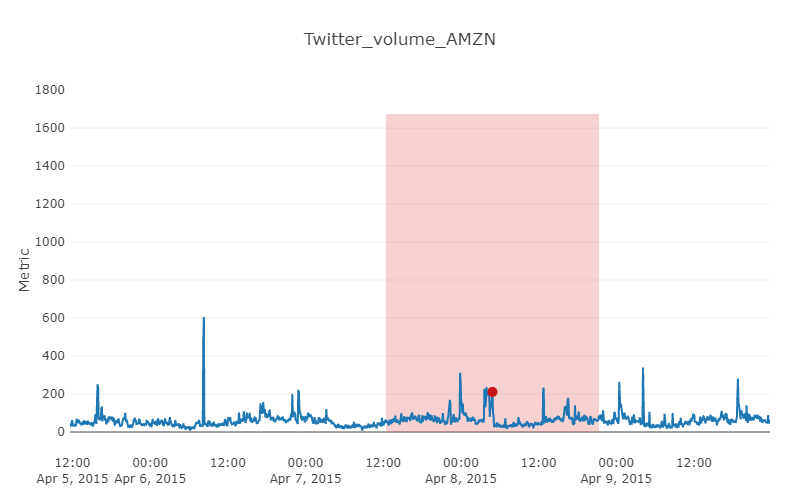
\includegraphics[width=.6\textwidth]{anomaly_windows.png}
        \caption{Example of an \defref{def:anomaly-window}. Illustration
        by the author.}\label{fig:anomaly-window}
    \end{figure}
\end{definition}
If multiple detections exist within a window, only the first detection is scored.
Additional detections within the window are ignored~\cite[cf.][]{Lavin.2015}.
Detections earlier in the window give higher positive scores than later detections.
Detections outside the anomaly window give negative scores.

Details on the calculation of the scoring function are given in \cref{app:numenta-score}
and an exemplary application is depicted in \cref{fig:anomaly-score-example}.


\paragraph{Visual Examination}
In this paragraph, an overview of the most common anomaly types within the \gls{nab}
is given. From visual observation only, the vast majority (about 30) of time
series from the dataset contain point anomalies~\cref{fig:point-anomalies-nab}.
Other more common types include contextual anomalies \cref{fig:contextual-anomalies-nab}.
Collective anomalies are only appear in form of change points. A very good example
as the one from \cref{fig:collective-anomalies-nab} is not contained in \gls{nab}.

Regarding triviality allegations from \textcite{Lavin.2015}, \(\sim 1/3\) of
point anomalies are so far from their neighborhood, that \(\mu_t + 3*\sigma_t\)
where \(\) would suffice to detect them, e.g.\ \cref{fig:point-anomalies-nab}.
This implies triviality of the dataset. However, such trivial solution would
also detect many false positives. While, from short examination, it should be
possible to solve many of the time series presented in \gls{nab} with
comparatively simple statistical operations, this solution would be unique for
every time series. Thereby defeating the purpose of \gls{nab} of scoring a
unified algorithm that must \textit{not} be adjusted for every such time series.

Additional plots from the dataset can be found in \cref{sect:additonal-plots-dataset}.

\begin{figure}[htp!]
    \centering
    \begin{subfigure}[t]{.49\linewidth}
        \centering
        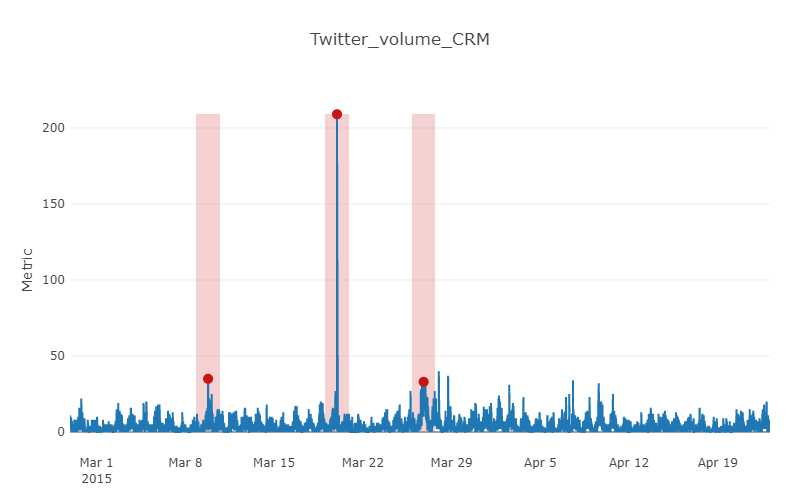
\includegraphics[width=\textwidth]{anomaly_types_examples/final/png/Twitter_volume_CRM.png}
        \subcaption{\footnotesize{}Point anomalies: Twitter\_volume\_CRM.csv}
    \end{subfigure}
    \begin{subfigure}[t]{.49\linewidth}
        \centering
        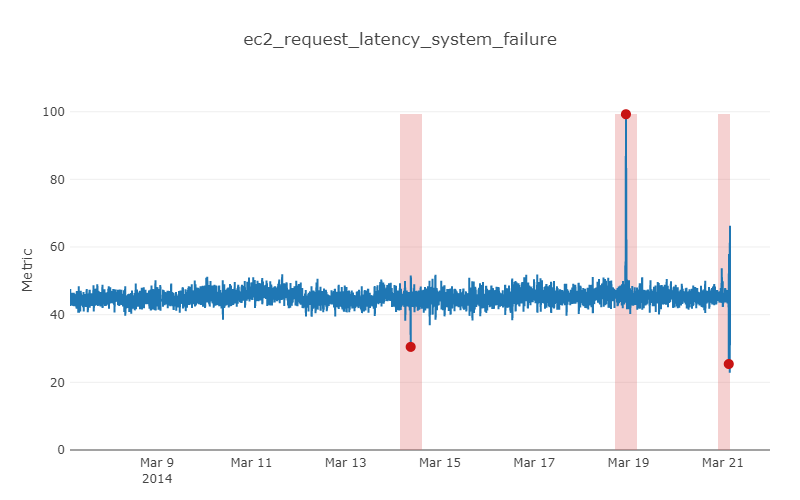
\includegraphics[width=\textwidth]{anomaly_types_examples/final/png/ec2_request_latency_system_failure.png}
        \subcaption{\footnotesize{}ec2\_request\_latency\_system\_failure.csv}
    \end{subfigure}
    \caption{Two examples of Point Anomalies}\label{fig:point-anomalies-nab}
\end{figure}

\begin{figure}[htp!]
    \centering
    \begin{subfigure}[t]{.49\linewidth}
        \centering
        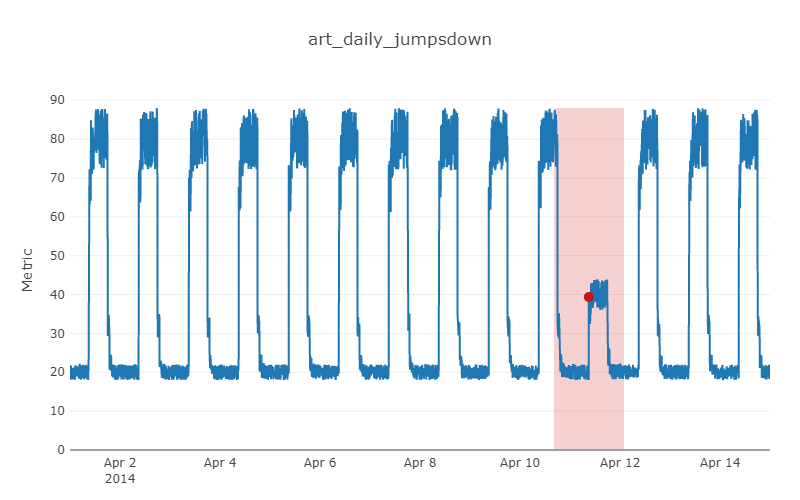
\includegraphics[width=\textwidth]{anomaly_types_examples/final/png/art_daily_jumpsdown.png}
        \subcaption{\footnotesize{}Point anomalies: art\_daily\_jumpsdown.csv}
    \end{subfigure}
    \begin{subfigure}[t]{.49\linewidth}
        \centering
        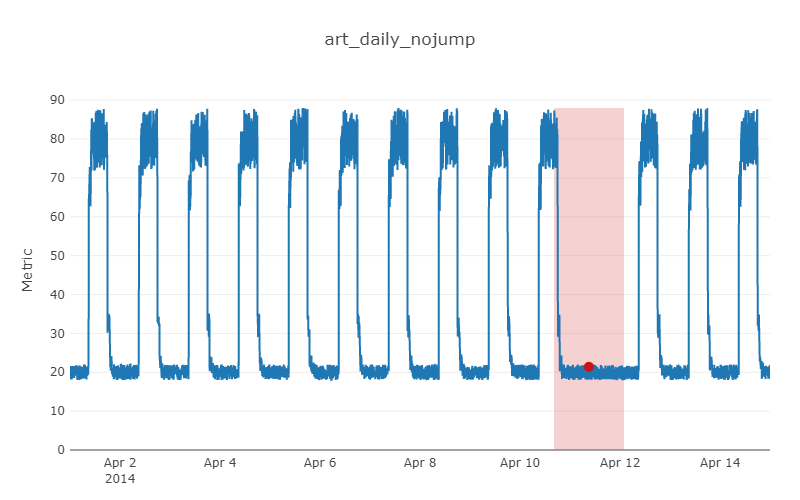
\includegraphics[width=\textwidth]{anomaly_types_examples/final/png/art_daily_nojump.png}
        \subcaption{\footnotesize{}art\_daily\_nojump}
    \end{subfigure}
    \caption{Two examples of (artificial) cyclicity violations (contextual anomalies)}\label{fig:contextual-anomalies-nab}
\end{figure}

\begin{figure}[htp!]
    \centering
    \begin{subfigure}[t]{.49\linewidth}
        \centering
        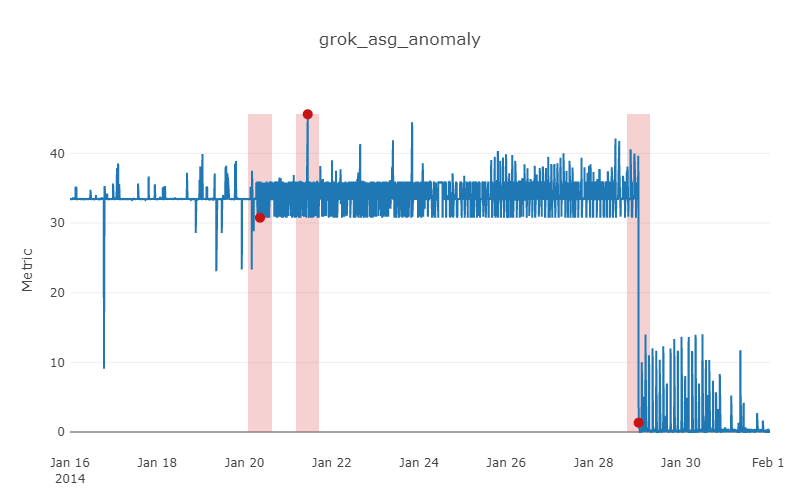
\includegraphics[width=\textwidth]{anomaly_types_examples/final/png/grok_asg_anomaly.png}
        \subcaption*{grok\_asg\_anomaly.csv}
    \end{subfigure}
    \caption{An example of two change points (collective anomalies) and a point anomaly}\label{fig:collective-anomalies-nab}
\end{figure}\todo{Is clearpage still required?}
\clearpage

\subsection{Algorithm overview}
In an attempt to reduce the implementation complexity required for this paper,
the majority of algorithms has been adopted from open source libraries and
adjusted slightly for application to the \gls{nab} dataset. On GitHub, several
repositories can be found which curate lists of such libraries. All repositories
used for this process are listed in \cref{tab:curation-lists}.

From these repositories, all libraries that offer algorithms belonging to either
\invdefref{def:forecasting-based-algo} or \invdefref{def:boundary-based-algo}
are listed in the appendix (forecasting-based: \cref{def:forecasting-based-algo},
boundary-based: \cref{tab:ad-packages}). Both tables contain an (almost exhaustive)
list of models offered by the library, the latest released version, and the date
of the latest commit.

Then, a subset of ten libraries is chosen, five of them with a focus on forecasting
and the remaining five with a focus on boundaries. Libraries that are encapsulated
in others are dropped from the list (e.g.\ \(\text{Prophet, GluonTS } \in \text{ AtsPy}\)).
Finally, the libraries are picked by the author, whereby recently updated libraries,
libraries with sufficient documentation and libraries with a high number of
stars (measuring to an extent the appreciation of the community) are slightly
preferred. The chosen libraries are presented in \cref{tab:chosen-packages}.

From these ten libraries, a subset of algorithms is selected. The selected
forecasting-algorithms are shown in \cref{tab:chosen-forecasting-algo},
boundary-algorithms are shown in \cref{tab:chosen-boundary-algo}.

If not stated otherwise, default parameters from within the libraries are adopted.
